\documentclass{beamer}
\usetheme{Boadilla}

\title{CONTROL SYSTEMS}
\author{by EE18BTECH11044}
\date{February 2020}

\usepackage{graphicx}

\begin{document}

\maketitle

\begin{frame}
\frametitle{Table of Contents}
\tableofcontents
\end{frame}

\section{Problem Statement}
\begin{frame}{Problem Statement}
Q) The transfer function C(s) of a compensator is given below.
\[C(s) = \frac{(1+\frac{s}{0.1})(1+\frac{s}{100})}{(1+\frac{s}{1})(1+\frac{s}{10})}\]
The frequency range in which the phase (lead) introduced by the compensator reaches the maximum is
\end{frame}
\section{Theory}

\begin{frame}{Theory}
\framesubtitle{Introduction}
\begin{itemize}
    \item In order to obtain the desired performance of the system, we use compensating networks. 
    \item Compensating networks are applied to the system in the form of feed forward path gain adjustment.
    \item Compensate a unstable system to make it stable.
    \item Compensating networks can also increase the steady state accuracy of the system.
    \item The three types of compensators — lag, lead and lag-lead are most commonly used electrical compensators.
\end{itemize}
Now let us see what lag, lead and lag-lead compensators briefly.
\end{frame}

\begin{frame}{Theory}
  \framesubtitle{Phase lead compensator}
\begin{itemize}
\item  A system which has one pole and one dominating zero (the zero which is closer to the origin than all over zeros is known as dominating zero.) is known as lead network. 
\item The phase-lead compensator adds positive phase to the system over the frequency range 1/ $\alpha$ T to 1/T. 
\end{itemize}
\begin{figure}[h]
\centering
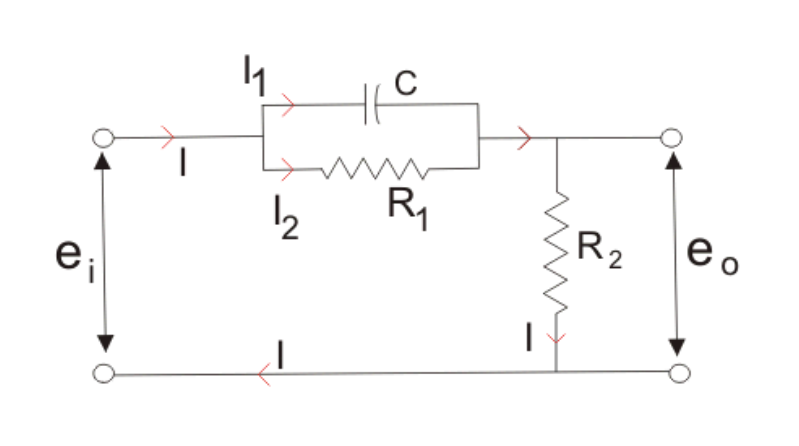
\includegraphics[width=4cm]{Screenshot (25).png}
\end{figure}
The transfer function of phase lead compensator is given by
\[Transfer Function = (\frac{1+\alpha s T}{1+s T})\]
%where alpha = (R_1 + R_2)/ R_2 and T = (R_1 R_2) /R_1+R_2
\end{frame}


\begin{frame}{Theory}
\framesubtitle{Phase lead compensator}
  \begin{figure}[h]
\centering
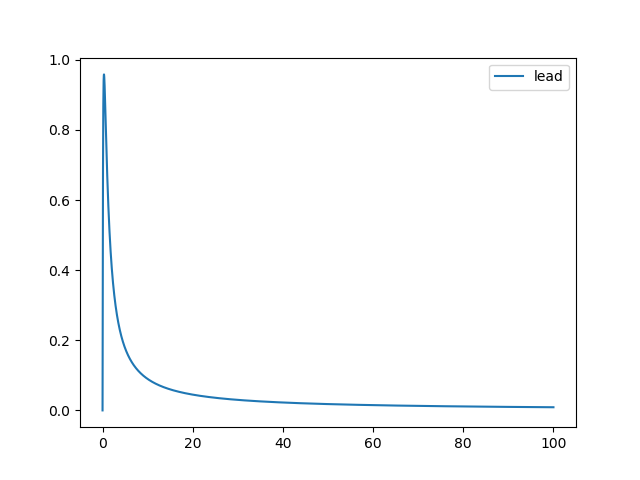
\includegraphics[width=9cm]{lead.png}
\caption{Phase plot for a phase lead compensator}
\end{figure}
\end{frame}

\begin{frame}{Theory}
\framesubtitle{Phase lag compensator}
\begin{itemize}
\item A system which has one zero and one dominating pole ( the pole which is closer to origin that all other poles is known as dominating pole) is known as lag network.
\item The phase-lag compensator adds negative phase to the system over the frequency range 1/T to 1/$\beta$T
\end{itemize}
\begin{figure}[h]
\centering
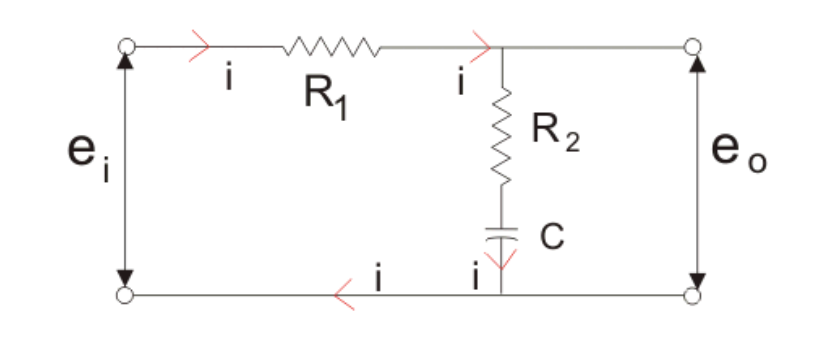
\includegraphics[width=4cm]{Screenshot (26).png}
\end{figure}
The transfer function of phase lag compensator is given by
\[Transfer Function = \frac{1}{\beta}(\frac{1+\beta s T}{1+ s T})\]
\end{frame}

\begin{frame}{Theory}
\framesubtitle{Phase lag compensator}
\begin{figure}[h]
\centering
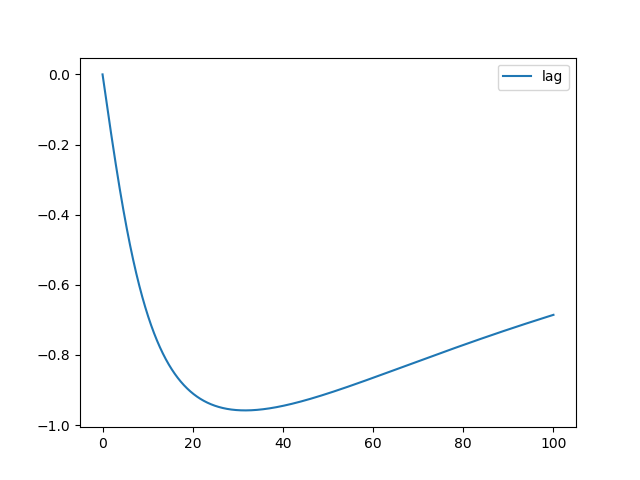
\includegraphics[width=9cm]{lag.png}
\caption{Phase plot for a phase lag compensator}
\end{figure}

\end{frame}

\begin{frame}{Theory}
\framesubtitle{Phase lag-lead compensator}
With single lag or lead compensation design specifications may not satisfied. For an unstable uncompensated system, lead compensation provides fast response whereas lag compensation stabilize the system. So we need multiple compensators in cascade.
\\
Given below is the circuit diagram for the phase lag- lead compensation network.
\begin{figure}[h]
\centering
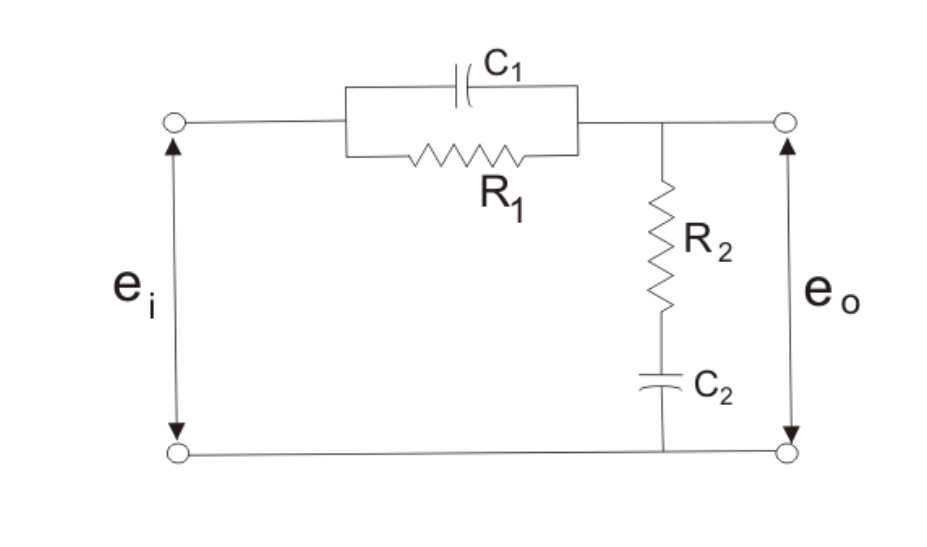
\includegraphics[width=4cm]{Screenshot (27).png}
\end{figure}
The transfer function of phase lag-lead compensator is given by
\[Transfer Function = \frac{(1+ \alpha s T_1)(1+\beta s T_2)}{(1+ s T_1)(1+s T_2)}\]
\end{frame}
\begin{frame}{Theory}
\begin{itemize}
\item Lead and lag compensators are used quite extensively in control. A lead compensator can increase the stability or speed of response of a system. 
\item lag compensator can reduce (but not eliminate) the steady-state error.
\item Generally $\alpha > 1$ and $\beta < 1$.
\item In a phase lead network pole is farther from origin than zero.
\item In a phase lag network zero is farther from origin than pole.
\end{itemize}

\end{frame}

\section{Solution}


\begin{frame}{Solution}
The given transfer function is :
\[C(s) = \frac{(1+\frac{s}{0.1})(1+\frac{s}{100})}{(1+\frac{s}{1})(1+\frac{s}{10})}\]
\[C(s) = \frac{(1+0.01 s)(1+10 s)}{(1+ 0.1 s)(1+ s)}\]
\begin{itemize}
\item Clearly the given transfer function is of a Phase lag-lead compensator.
\item Comparing the equations, we get $\alpha$ = 10 , $T_1$ = 1 , $\beta$ = 0.1 and   $T_2$ = 0.1 .

\item The pole zero diagram for the given compensator transfer function would be :
\end{itemize}
\end{frame}

\begin{frame}{Solution}
\begin{figure}
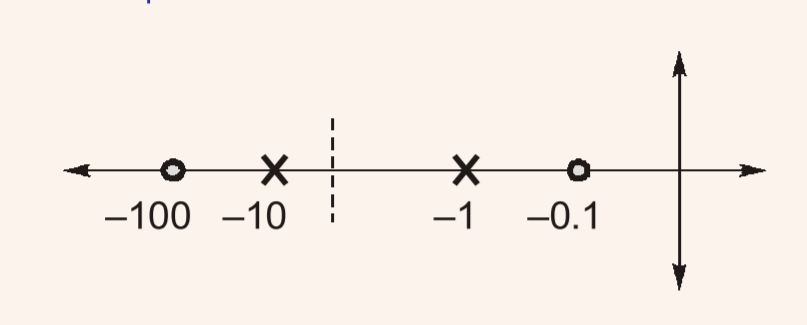
\includegraphics[width=8cm]{Screenshot (30).png}
\end{figure}
\begin{itemize}
    \item In the above pole zero plot the pole-zero pair closer to the origin corresponds to phase lead part and pole-zero pair away from origin corresponds to the phase lag part.
    \item The frequency range in which the phase(lead) introduced by the compensator reaches maximum will be when phase lead part is dominating over the phase lag part.
    \item This will occur when $\omega$ ranges between 0.1 and 1.
\end{itemize}
\end{frame}
\section{Verification}
\begin{frame}{Verification}
Plotting the phase of transfer function as a function of $\omega$. 
\begin{figure}
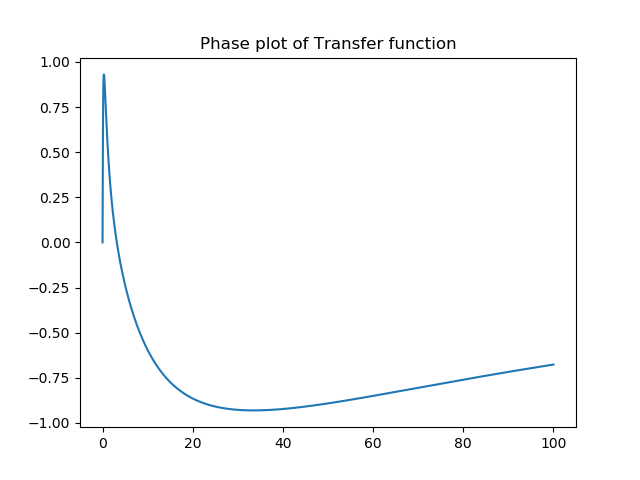
\includegraphics[width=8cm]{ptotal.png}
\end{figure}
\end{frame}

\begin{frame}{Verification}
Limiting the axis from 0 to 2, we can clearly observe the maxima between 0.1 and 1. 
\begin{figure}
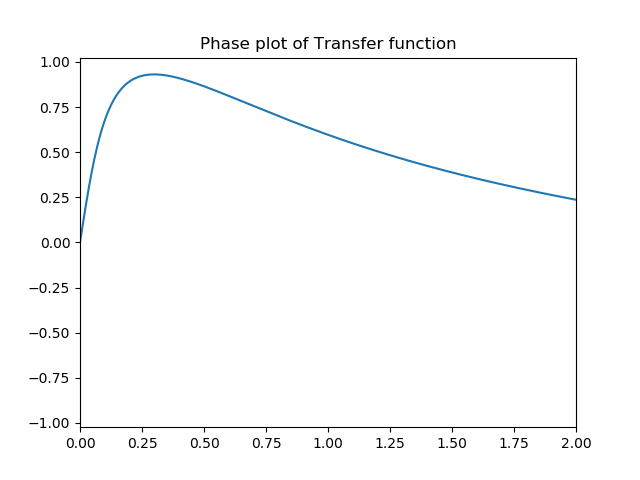
\includegraphics[width=8cm]{puntil2.png}
\end{figure}
\end{frame}


\begin{frame}
\huge{\centerline{The End}}
\end{frame}

\end{document}
